\section{Background}
Include a few words here about the background and motivation of the project. 

This can be helped by explaining what has happened in the past; what you are going to do in the present; and how this action will help and change the future. 



\section{Aims}
This should be a general aim of the overall project. This should be explained in one or two paragraphs.

\subsection{Objectives}
These are a list of clearly defined objectives that can be aligned to outcomes in the project. We can define the success of the project based on these fulfilling these objectives.
\begin{itemize}
\item Research
\item Explore Hypotheses
\item Design Experimental Framework
\item Run experiments under Experiment Framework and test hypotheses
\item Analyse Results
\item Provide detailed recommendations and guidelines 
\end{itemize}


\subsection{Deliverables}
Deliverables are a result of actions that complete and attempt to satisfy objectives and can include:
\begin{itemize}
\item Complete proposal
\item Complete Research Ethics approval
\item Complete research on specified related area
\item Complete research on another specified related area
\item Complete Literature Review
\item Conduct Experiments under completed Designed Experimental Framework
\item Complete Software Development
\item Complete Experiments based on Experimental Framework
\item Collate and gather information and data from Experiments
\item Analyse Results and complete write-up of results
\item Complete Conclusions
\item Complete Turn-it-in submission
\item Print, bind and submit two hard copies to Unihelpdesk.
\end{itemize}

\section{Resources}
List any software or hardware that may be required for the completion of the project.

\begin{itemize}
\item Forensic ToolKit
\item The Sleuth Kit
\item Laptop
\item 10 1Gb memory sticks
\item 2 128Gb SSD
\item FTK Imager
\end{itemize}

\section{Schedule}
Typically include a GANTT chart indicating when the objectives and deliverables are met.

This can be completed by Excel or other dedicated software and then imported into this document as shown in Fig.\ref{fi:GANTT}.



% % % % % % % % % % % % % % %
%
%	INCLUDING FILES	
%	File: ch1/gantt.png
%	N.B. 	This is compiled from the parent directory.
%		Hence referencing ch1 directory from within ch1
% 
% % % % % % % % % % % % % % %
\begin{figure}
\centering
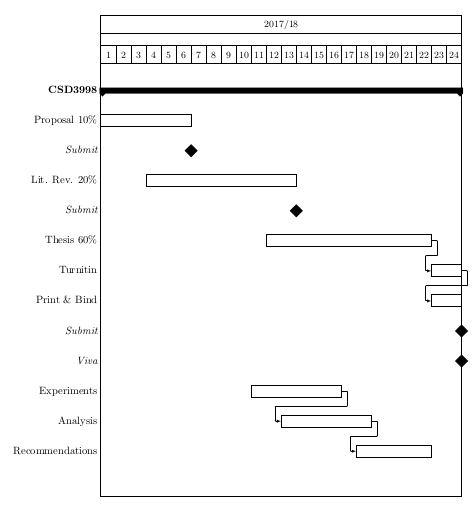
\includegraphics[scale=0.4]{ch1/gantt}
\caption{GANTT Chart showing indicative milestones.}\label{fi:GANTT}
\end{figure}


\section{Summary}

Optional, but this section could outline and emphasise the structure of the thesis. It could also be used to emphasise what the project is about and can sometimes be used to disambiguate any areas, e.g., your project may look into applying text mining to e-discovery and you may want to emphasise that this is an application and not a project on text mining.

The structure of the rest of this thesis (never refer to the thesis as a paper and always write in third person) is as follows: Chapter 2 covers the literature review and current research related to the problem; Chapter 3 investigates the experiment and rationalises the method undertaken; Chapter 4 analyses the results; and Chapter 5 includes the recommendations and conclusions. 


